\chapter{Effects of beet juice}
% ------------------------
% ------------------------
\section{Beetroot juice and the nitric oxide pathway}
% ------------------------
Early work by Bailey et al showed that supplementation of beetroot juice reduced the oxygen cost of submaximal exercise, and increase athletes' time to exhaustion\cite[1]{bailey2009dietary}. These remarkable effects have been traced back to beetroot juice's tendency to increase nitric oxide ($\mathrm{NO}$) within in the bloodstream.

There are two pathways by which nitric oxide is produced within the body. The first is endogenous, and results from an oxidation reaction of the amino acid L-arginine and the enzyme NOS\cite[1]{boorsma2013effect}\cite[1]{lundberg2008nitrate}.

However, it is the second $\mathrm{NO}$ pathway which is of interest in this paper. 
In this process, illustrated in Figure \ref{fig:dominguez}, $\mathrm{NO}$ is can be produced through a double reduction reaction of nitrate, \notm. Beetroot juice is known to be a uniquely high source of dietary \notm\cite{bailey2009dietary}. 

Dietary nitrate, when consumed, is absorbed into the bloodstream. From there, the nitrate is reduced, yielding nitrite, \nottm, by bacteria in the mouth\footnote{It is worth noting that these bacteria are critical to the conversion process. Many of the studies references in this literature forbit their test subject from using mouthwash for the duration of the study period. It has been demonstrated that interfering with the bacterial cultures would prevent the conversion of nitrates\cite{govoni2008increase}.}. This nitrite is then ``physiologically recycled"\cite[1]{lundberg2008nitrate}, and absorbed again into the bloodstream, through the salivary gland, and then into the stomach. Immediately upon reaching the stomach, the bulk of the \nottm is reduced, yielding $\mathrm{NO}$.

Nitric oxide has several uses in the body. For the purposes of this article, the key contribution of $\mathrm{NO}$ is its tendency to reduce the oxygen cost of aerobic exercise. $\mathrm{NO}$ can effectively act to replace oxygen molecules in the Complex IV reaction in the electron transport chain \cite[19]{boorsma2013effect}--remarkably reducing the physiological oxygen cost of exercise.

\begin{figure}[h]
    \centering
    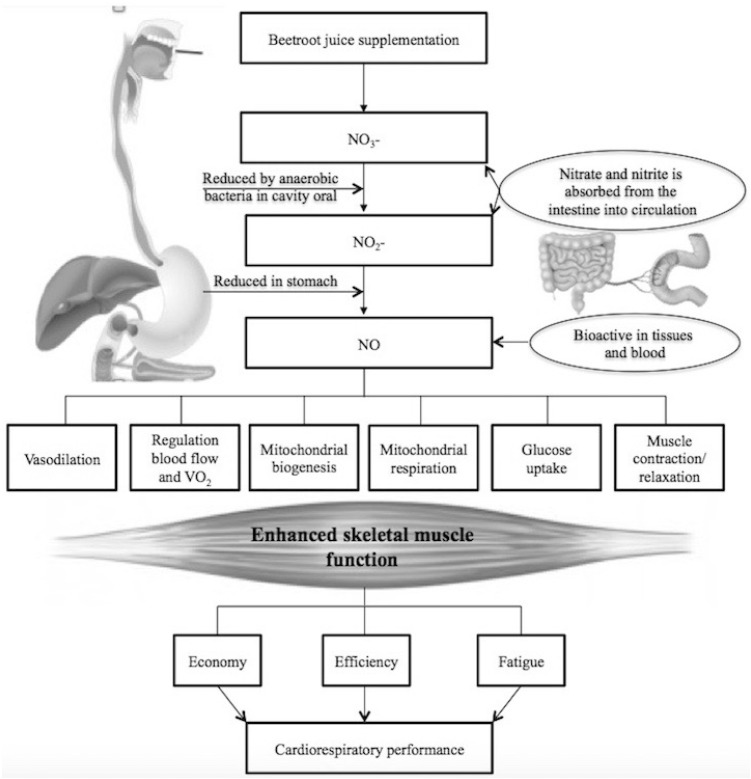
\includegraphics[width=0.9\textwidth]{assets/dominguezfigure.jpg}
    \caption{Illustration showing the endogic  conversion of nitric oxide as a result of oral beetroot juice intake. Retrieved from Dominguez et al \cite{dominguez2017effects}.}
    \label{fig:dominguez}
\end{figure}
% ------------------------
% ------------------------
\section{Elite runners}
A double-blind, placebo-controlled crossover study from the University of Guelph presented the first findings on the effect of beetroot juice to elite-level male distance runners\cite[56]{boorsma2013effect}.

The study tracked male ($n=8$) subjects in an 8-day period, with data obtained following an acute dose, as well as after 8 days of chronic supplementation of either a placebo or a high-nitrate beetroot juice. Subjects were tested for plasma \notm concentration, and running efficiency (\vot, \vcot, RER, and HR) through a submaximal treadmill test followed by an individual \SI{1500}{m} time trial on an indoor track\cite[40]{boorsma2013effect}.

Within 90 and 150 minutes of a single dose, the subjects showed significantly elevated levels of plasma \notm (\SI{37\pm15}{\micro M} at baseline, \SI{615\pm151}{\micro M} 90min after dose, \SI{596\pm64}{\micro M} 150min after dose). 

Despite the great increase in plasma \notm, Boorsma concluded that the beetroot juice supplement produced no statistically significant effect on any of the perfomance quantifiers\cite[63]{boorsma2013effect}. The \SI{1500}{m} time trials showed no significant difference or order effect across the four trials (acute placebo, chronic placebo, acute supplement, chronic supplement). Similarly, the treadmill tests yielded no significant changes in \vot, \vcot, RER, and HR\cite{boorsma2013effect}.

Boorsma did note that 2 out of the 8 subjects did respond to the beetroot juice supplement to a higher degree than average \cite[69]{boorsma2013effect}. These two subjects showed an improvement in their \SI{1500}{m} time trial that exceeded the coefficient of variation for elite males at this distance\cite[60]{boorsma2013effect}, which suggests that the supplement may have a meaningful effect on their performance. Boorsma notes that these two athletes were on the lower (but not bottom) end of the performance range for the surveyed athletes, and suggests that their improvement may come as a result of their lesser physical training adaptations relative to the other subjects\cite[61]{boorsma2013effect}. It may also be possible that some fraction of elite athletes do respond well to beetroot juice supplementation. A study done on elite cyclists in 2012 elicited a similar response: 2 out of 8 elite cyclists showed a reduction in \vot at medium and low intensity efforts\cite[8]{christensen2013influence}. More research is necessary to determine the cause, but Christensen notes that the composition of fast versus slow twitch muscle fibers could be one possible factor\cite[8]{christensen2013influence}.

Balsalobre-Fern\'andez, from the Universidad Aut\'onoma de Madrid, conducted a study on elite male runners $(n=12)$ training at the High Performance Center of Madrid. Athletes were given either a beetroot juice supplement (or a placebo) to consume for a period of 15 days.

Eight variables were tracked in each subject: RPE, muscle oxygen saturation, RER, \vot{} and \votmax, heart rate, \tex{} (time to exhaustion), and leg stiffness. The study finds that statistically significant effects were only found for RPE, \smo, and \tex. These variables showed improvements (as measured in standardized mean differences between placebo and experimental and 90\% confidence interval) of
${-2.17\,(-3.23,-1.1)}\ \SI{}{\textrm{out of 10}}$,
${0.72\,(0.03,1.41)}\ \SI{}{\%}$,
${1.18\,(-0.14,2.5)}\ \SI{}{s}$,
respectively.
All remaining variables showed an unclear relationship to beetroot juice consumption in comparison to the effects observed in the placebo group. 

It is worth noting that the variables which do indicate a possible relationship with beetroot juice supplementation in the Balsalobre study are not tracked in Boorsma's study, so no comparison can be made. However, both studies agree that there is no clear relationship between beetroot juice supplementation in elite male runners with respect to \vot{},\votmax, and RER (and therefore also not in running economy). These results are consistent with prior findings in studies on elite athletes from other sports, such as flatwater kayaking\cite{muggeridge2013effects} and cycling\cite{christensen2013influence} in concluding that beetroot juice does not appear to enahance  performance in elite athletes.

% ------------------------
\section{Recreational runners}
Studies indicate that recreational athletes may benefit from both chronic consumption as well as acute consumption. A review by Dominguez states that acute supplementation of beetroot juice within 2-3 hours of exercise reduces oxygen consumption (at or below \votmax{} intensity), increases time to exhaustion, and may improve performance at \votmax{} intensity\cite[13]{dominguez2017effects}.

A study from Brazil, by Fernandes  de  Castro, tested a group of 14 male runners for maximum HR, RPE, \SI{10}{km} run time trial, glycogen, and maximum lactate concentration following baseline, chronic supplementation, or a placebo\cite[19]{de2019effect}. In this case, the chronic supplementation was only three days. The study concluded that none of the variables had a statistically significant relationship to beet juice supplementation\cite{de2019effect}. This is not necessarily in disagreement with the literature, since the review by Dominguez does not claim that beetroot juice improves those particular variables \cite{dominguez2017effects}.
With regards to the \SI{10}{km} results: it should be noted that less experienced athletes may not pace themselves optimally during a race effort, and thus the conditions are uncontrolled in this regard. This is shown in the study, as most subjects began their effort too fast and dropped their pace with each subsequent kilometer\cite[20]{de2019effect}.  Using a controlled experiemental setup consisting of a treadmill, and analyzing \vot{} would enable the observation of more precise results.
%\section{Comparison of results}
%Table \ref{tab:summary} displays an overview of results obtained by the body of research.
%\begin{table}[]
%    \centering
%    \begin{tabular}{lll}
%    \hline
%    Performance metric  & Elite   & Recreational %\\\hline
%    \votmax  &  &  \\
%    RPE  &  &  \\
%    \hline
%    \end{tabular}
%    \caption{Summary of results obtained by researchers.}
%    \label{tab:summary}
%\end{table}